

\tikzset{every picture/.style={line width=0.75pt}} %set default line width to 0.75pt        

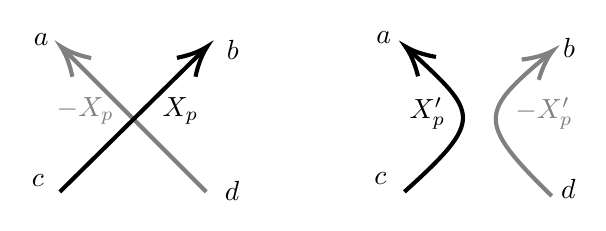
\begin{tikzpicture}[x=0.75pt,y=0.75pt,yscale=-1,xscale=1]
%uncomment if require: \path (0,109); %set diagram left start at 0, and has height of 109

%Straight Lines [id:da7979059503936952] 
\draw [color={rgb, 255:red, 128; green, 128; blue, 128 }  ,draw opacity=1 ][line width=1.5]    (39.62,19.12) -- (107.5,87) ;
\draw [shift={(37.5,17)}, rotate = 45] [color={rgb, 255:red, 128; green, 128; blue, 128 }  ,draw opacity=1 ][line width=1.5]    (14.21,-6.37) .. controls (9.04,-2.99) and (4.3,-0.87) .. (0,0) .. controls (4.3,0.87) and (9.04,2.99) .. (14.21,6.37)   ;
%Straight Lines [id:da7279842833116223] 
\draw [color={rgb, 255:red, 0; green, 0; blue, 0 }  ,draw opacity=1 ][line width=1.5]    (105.86,19.11) -- (37,87) ;
\draw [shift={(108,17)}, rotate = 135.41] [color={rgb, 255:red, 0; green, 0; blue, 0 }  ,draw opacity=1 ][line width=1.5]    (14.21,-6.37) .. controls (9.04,-2.99) and (4.3,-0.87) .. (0,0) .. controls (4.3,0.87) and (9.04,2.99) .. (14.21,6.37)   ;
%Curve Lines [id:da5605408166706283] 
\draw [color={rgb, 255:red, 0; green, 0; blue, 0 }  ,draw opacity=1 ][line width=1.5]    (203,87) .. controls (242.2,51.72) and (238.18,49.09) .. (205.53,18.88) ;
\draw [shift={(203.5,17)}, rotate = 402.85] [color={rgb, 255:red, 0; green, 0; blue, 0 }  ,draw opacity=1 ][line width=1.5]    (14.21,-6.37) .. controls (9.04,-2.99) and (4.3,-0.87) .. (0,0) .. controls (4.3,0.87) and (9.04,2.99) .. (14.21,6.37)   ;
%Curve Lines [id:da8925010918239024] 
\draw [color={rgb, 255:red, 128; green, 128; blue, 128 }  ,draw opacity=1 ][line width=1.5]    (274,89) .. controls (236.76,52.74) and (239.86,48.17) .. (272.47,20.71) ;
\draw [shift={(274.5,19)}, rotate = 499.95] [color={rgb, 255:red, 128; green, 128; blue, 128 }  ,draw opacity=1 ][line width=1.5]    (14.21,-6.37) .. controls (9.04,-2.99) and (4.3,-0.87) .. (0,0) .. controls (4.3,0.87) and (9.04,2.99) .. (14.21,6.37)   ;

% Text Node
\draw (23,9.4) node [anchor=north west][inner sep=0.75pt]    {$a$};
% Text Node
\draw (116,12.4) node [anchor=north west][inner sep=0.75pt]    {$b$};
% Text Node
\draw (22,77.4) node [anchor=north west][inner sep=0.75pt]    {$c$};
% Text Node
\draw (115,80.4) node [anchor=north west][inner sep=0.75pt]    {$d$};
% Text Node
\draw (85,40) node [anchor=north west][inner sep=0.75pt]  [color={rgb, 255:red, 0; green, 0; blue, 0 }  ,opacity=1 ]  {$X_p$};
% Text Node
\draw (34,40) node [anchor=north west][inner sep=0.75pt]  [color={rgb, 255:red, 128; green, 128; blue, 128 }  ,opacity=1 ]  {$-X_p$};
% Text Node
\draw (188,8.4) node [anchor=north west][inner sep=0.75pt]    {$a$};
% Text Node
\draw (278,11.4) node [anchor=north west][inner sep=0.75pt]    {$b$};
% Text Node
\draw (187,76.4) node [anchor=north west][inner sep=0.75pt]    {$c$};
% Text Node
\draw (277,79.4) node [anchor=north west][inner sep=0.75pt]    {$d$};
% Text Node
\draw (204,40) node [anchor=north west][inner sep=0.75pt]  [color={rgb, 255:red, 0; green, 0; blue, 0 }  ,opacity=1 ]  {$X'_p$};
% Text Node
\draw (255,40) node [anchor=north west][inner sep=0.75pt]  [color={rgb, 255:red, 128; green, 128; blue, 128 }  ,opacity=1 ]  {$-X'_p$};


\end{tikzpicture}